\chapter{Markov Chains and Generalities}
\textbf{Framework}: $(\Omega, F, \mathbb{P})$ Probability Space, $E$ finite or countable set with the $\sigma$-algebra $2^E$

\noindent
\textbf{Outset} We would like to define a class of processes such that the evolution of the process is memoryless, but still location dependent. This means that the way a process continues past this point in time, does not depend on how it got to where it is now, but only on where it is at this point in time. 

\begin{defn}
	A sequence $X_n, n \in \mathbb{N}$ of RVs with values in $E$ is a homogeneous time Markov Chain (MC) if:
\begin{enumerate}
	\item  For all $n \geq 0$ and $x_1,\ldots,x_{n+1} \in E$
\begin{align}
	\quad \boxed{\mathbb{P} \left[ X_{n+1}=x_{n+1} | X_0=x_0,\ldots,X_n=x_n \right] = \mathbb{P} \left[ X_{n+1}=x_{n+1} | X_n = x_n \right]}
\end{align}
	\item For all $m,n \geq 0$ and $x,y \in E$
\begin{align}	
	\boxed{\mathbb{P} \left[ X_{n+1}=y | X_{n}=x \right] = \mathbb{P} \left[ X_{n+1=y}| X_n=x \right]} 
\end{align}
\end{enumerate}

\end{defn}


By convention when we write $\mathbb{P} \left[ A|B \right] $ we assume $\mathbb{P} \left[ B \right] >0$.

\begin{rmk}
The first condition is equivalent to for all $f:E\to \mathbb{R}$ bounded, $\mathbb{E} \left[ f(X_{n+1}) | X_0,\ldots,X_n \right] = \mathbb{E} \left[ f(X_{n+1}) | X_n \right] $
\end{rmk}

\begin{ex}
	If $X_n$ are iid in $E$ then $X_n$ is a MC
\end{ex}

\begin{ex}
	SRW on $\mathbb{Z}^d$
\end{ex}

\section{Transition Probabilities}
\textbf{Motivation} In a finite state space $E=\{1,2,3\}$, then we write the probability to go from 1 to 2 as $p_{12}$. We would like to write these probabilities in a matrix.

\begin{defn}
	A transition probability is a collection $p=(p_{x,y})_{x,y \in E}$ such that:
	\begin{itemize}
		\item For any $x,y \in E$: $p_{x,y}\in [0,1]$ 
		\item $\sum_{y \in E} p_{x,y}=1$
	\end{itemize}
	
\end{defn}

We could also represent this as a weighted directional graph with vertices $E$ and weighted oriented edges: $\{(x,y) \in E: p_{x,y}>0\}$. We know there is a 1 to 1 correspondence between directional graphs and matrices.

\textbf{Matrix} So say $E=\{1,\ldots,N\}$ and $p=(p_{ij})_{1\leq i,j\leq N}$ with $p_{ij}\geq 0$ and $\sum_{j}p_{ij}=1$. We call this a stochastic matrix.

\textbf{Operator} If $E$ is finite or infinite then $\forall f \in L^\infty (E)$ define $Pf \in L^\infty (E)$ by  $Pf(x)=\sum_{y \in E}P_{x,y}f(y)$ with $P\geq 0 $ ($\forall  f \geq 0: Pf \geq 0$ ) and satisfies $P1=1$.

\begin{defn}
	Let $p$ be a transition probability, $\psi$ distribution on $E$, a sequence $(X_n)_{n\geq 0}$ of RVs with values in $E $ is a Markov Chain with initial distribution $\mu$ and transition probability $p$ (written $ \textrm{MC}(\psi, p)$) if for $x_0, \ldots, x_n \in E$
\begin{align}
	\boxed{ \mathbb{P} \left[ X_0=x_0, \ldots ,X_n=x_n \right] = \mu(x_0)p_{x_0,x} \cdots p_{x_{n-1},x_{n}} }
\end{align}

\end{defn}

\begin{prop}
	Let $(X_n)_{n \geq 0}$ sequence of RVs with values in $E$:
	$(X_n)_{n \geq 1}$ is a MC $\iff$ $\exists \mu, p$ such that $(X_n)_n$ is a MC$(\mu, p)$
\end{prop}
\begin{proof}
	$\implies:$ If $X_n$ is a MC, then set $p_{xy}=\mathbb{P}_{} \left[ X_{n+1}=y | X_{n}=x \right] $. $\sum_{y \in E}^{} p_{xy}=1$, as the conditional probability is a probability measure itself, and $p_{xy}\geq 0, \forall x, y \in E$ for the same reason. Thus we have that the collection of $(p_{xy})_{x,y \in E}$ form a transition probability. Setting $\mu(x) = \mathbb{P}_{} \left[ X_0 =x \right] $, which is also clearly a probability measure on $E$. Now we only have to show that $X_{n} $ is a $ \textrm{MC}(\mu, p)$. For every $x_0,\ldots , x_n \in E$, and every $n\geq 0$, we have
\begin{align}
	\mathbb{P}_{} \left[ X_0=x_0, \ldots ,X_n=x_n \right]  
	&= \mathbb{P}_{} \left[ X_n = x_n | X_0=x_0 , \ldots , X_{n-1}=x_{n-1} \right] \mathbb{P}_{} \left[ X_0=x_0 , \ldots , X_{n-1}=x_{n-1} \right] \\
	&= \mathbb{P}_{} \left[ X_0 = x_0 \right] \prod_{i=1}^{n} \mathbb{P}_{} \left[ X_i = x_i | X_0=x_0, \ldots , X_{i-1}=x_{i-1} \right] \\
	&= \mu(x_0) \prod_{i=1}^n \mathbb{P}_{} \left[ X_i = x_i | X_{i-1} = x_{i-1}  \right] = \mu(x_0) \prod_{i=1}^n p_{x_{i-1}x_{i}} 
\end{align}
Thus we have proven this implication, by using the Markov Property of Markov Chains.

$\impliedby:$ Here we have to show the two aspects of a Markov chain, the Markov Property and homogeneity. For homogeneity we have
\begin{align}
&	\mathbb{P}_{} \left[ X_{n+1} = y | X_n =x \right] \\
&\qquad = \sum_{(u_0, \ldots ,u_{n-1}) \in E^n}^{} \mathbb{P}_{} \left[ X_{n+1}=y | X_0=u_0, \ldots ,X_{n-1}=u_{n-1}, X_n =x \right] * \\
& \qquad \qquad \qquad \qquad \qquad  \mathbb{P}_{} \left[ X_0=u_0, \ldots , X_{n-1}=u_{n-1} | X_n = x \right] \\
&\qquad = p_{xy} \sum_{(u_0, \ldots ,u_{n-1})\in E^n}^{} \mathbb{P}_{} \left[ X_0=u_0, \ldots ,X_{n-1}=u_{n-1} | X_n = x \right] = p_{xy}
\end{align}
here we have implicitly (sneakily) assumed that $\mathbb{P}_{} \left[ X_n = x \right] > 0$, as without this the conditional probability we are taking is not well-defined.

For the Markov Property we have
\begin{align}
	\mathbb{P}_{} \left[ X_{n+1} = x_{n+1} | X_0 =x_0, \ldots ,X_n=X_n \right] &=
		\frac{\mathbb{P}_{} \left[ X_0=x_0, \ldots , X_{n+1}=x_{n+1} \right] }
		{\mathbb{P}_{} \left[ X_0=x_0 , \ldots , X_{n}=x_{n} \right]} \\
	&= \frac{\mu(x_0)p_{x_0 x_1}  \cdots  p_{x_{n}x_{n+1}}} {\mu(x_0)p_{x_0x_1} \cdots p_{x_{n-1}x_{n}}} \\
	&= p_{x_n x_{n+1}} = \mathbb{P}_{} \left[ X_{n+1} = x_{n+1} | X_n=x_n \right] 
\end{align}
where it is important to note that, again,  we have implicitly assumed that \newline $\mu(x_0)p_{x_0x_1} \cdots p_{x_{n-1}x_n}>0$. 

\end{proof}


\textbf{Question} Given $\mu, p$ does $ \textrm{MC}(\mu, p)$ always exist (as a MC)?

\section{Existence}

\begin{theorem}
	Let $p$ be a transition probability on $E$. Then there exists:
\begin{enumerate}
	\item a measurable space $(\Omega, F)$
	\item a collection of probability measures $(P_x)_{x}$ on $(\Omega, F)$
	\item a sequence of RVs $(X_n)_{n \geq 0}$ on $(\Omega, F)$ such that for all $x\in E$, under $P_x$, $(X_n)$ is  $ \textrm{MC}(\delta_x, p)$
\end{enumerate}

\end{theorem}

There are 2 approaches to prove this. 

One could set $\Omega = E^{\mathbb{N}}, \quad \mathbb{P} \left[ (x_0, \ldots ,x_n) | x \in E^n \right] = \delta_x(x_0) p_{x_0,x_1} \cdots p_{x_{n-1},x_n}$.
Instead we will work as follows:
\begin{proof}
	We consider a measure $\mu $ on $E$ such that $\forall x \in E: \mu (x) >0$ on some abstract probability space (this part is of technical relevance) $(\Omega, \mathcal{F}, \mathbb{P} )$. Now we look at a RV $X_0$ with distribution $\mu$, and $U_1,U_2, \ldots $ independent, uniformly distributed, RVs on $[0,1]$ (we know these exist from previous probability lectures). Our goal is to use these uniform RVs to produce the probabilities given by the transition probabilities, in a way similar to Sklar's Theorem (knowledge of Sklar's is not needed here). To do this we enumerate $E=\{x_i, i \in I \}$ where $I$ is our index set (eg. $\{1,2, \ldots ,n\}$ or  $\mathbb{N}$) and set $s_{ij}= \sum_{k<j}p_{x_ix_k} $. Note here that $s_{i,j+1}-s_{i,j} = p_{x_ix_j} $. Finally, set $\Phi: E \times [0,1] \to E; (x_i,u) \mapsto x_j $ if $u \in (s_{i,j}, s_{i,j+1}]$, a measurable function. Now we have $X_0$ as needed and the tools to construct the sequence of RVs, along with the collection of probability measures we want.

	What these tools have given us is that $\mathbb{P}_{} \left[\Phi(x,U_1) = y  \right] = p_{xy}$. So if we set $X_{n+1} = \Phi(X_n, U_{n+1})$ for every $n>0$ (by induction), we find that
\begin{align}
	\mathbb{P}_{} \left[ X_0=x_0, \ldots ,X_n=x_n \right] &=
		\mathbb{P}_{} \left[ X_0=x_0, \Phi(x_0, U_1)=x_1 , \ldots , \Phi(x_{n-1}, U_{n}) = x_n \right] \\
	&= \mu(x_0)p_{x_0x_1} \cdots p_{x_{n-1}x_n}
\end{align}
by independence.

Now if we define $\mathbb{P}_{x} $ as $\mathbb{P}_{} \left[\ \cdot\ | X_0 = x_0 \right] $, then we have $\forall x \in E$ $\mathbb{P}_{x} \left[ X_0=x_0, \ldots ,X_n=x_n \right] = \delta_x(x_0)p_{x_0x_1} \cdots p_{x_{n-1}x_n}$.


\end{proof}


\noindent
\textbf{Framework for the rest of the chapter} 
$E$ is finite or countable, $p$ transition probability, $(\Omega, F, (P_x)_{x \in E})$ Prob. Spaces, $(X_n)_{n \geq 0}$ RV such that it is a  $ \textrm{MC}(\delta_x, p)$ under $P_x$.

For $\mu$ Prob measure on $E $ we write $P_\mu= \sum_{x}\mu(x)P_x$

\section{Simple Markov Property}
Under $P_\mu$ $(X_n)_{n \geq 0}$ is $ \textrm{MC}(\mu, p)$.
$P_\mu [X_{n+1}=x_{n+1} | X_0 = x_0, \ldots ,.X_n=x_n] = P_\mu[X_{n+1}=x_{n+1}| X_n = x_n] = P_{x_n}[X_1 =x_{n+1}]$ i.e. Conditional on $X_n=x$, $x_{n+1}$ is sampled like the first step of a $ \textrm{MC}(\delta_{x},p)$ indep of the past.

\textbf{Notation} $ \mathcal{F}_n = \sigma(X_0, \ldots ,X_n)$ 

\begin{theorem}[Simple Markov Property (SiMP)]
	Let $\mu$ be a distribution on E. Let $x \in E, k \in \mathbb{N}$. For every $f: E^{\mathbb{N}} \to \mathbb{R}_+$ measurable and bounded, for every $Z$ bounded which is $ \mathcal{F}_k$ measurable RV:

	$\mathbb{E}_\mu \left[ f((X_{k+n})_{n \geq 0})Z | X_k = x_k \right] = \mathbb{E}_{x_k} \left[ f((X_n)_{n \geq 0} \right] \mathbb{E}_\mu \left[ Z | X_k=x \right] $
\end{theorem}
\begin{proof}
	First note that using $Z= \mathbbm{1}_{X_0=x_0, \ldots ,X_{k-1}=x_{k-1}}$ we only have to prove that \newline $\mathbb{E}_{\mu } \left[ f((X_{k+n})_{n\geq 0}) | X_0=x_0 , \ldots , X_k=x_k \right]= \mathbb{E}_{x_k} \left[ f((X_n)_{n\geq 0}) \right]$. We will proceed using measure theoretic induction (see any book on measure theory). Approximate $f$ by step functions $f_k$, using linearity, we only have to show our claim for the function $\mathbbm{1}_{A} $ with $A \subset E ^{\mathbb{N}}$, i.e. 
	\begin{align}
	\mathbb{P}_{\mu } \left[ (X_{k+n})_{n\geq 0}\in A | X_0=x_0, \ldots ,X_k=x_k \right] = \mathbb{P}_{x_k} \left[ (X_n)_{n\geq 0} \in A \right] 
\end{align}  
The collection of sets of the form $A=\{w \in E^{\mathbb{N}}: w_0=y_0, \ldots ,w_N=y_N\}$ for $N\geq 0$ and $y_0, \ldots ,y_N \in E$ form a $\pi $ system generating our $\sigma$-algebra. Furthermore, on such sets 
\begin{align}
&	\mathbb{P}_{\mu } \left[ (X_{k+n})_{n\geq 0}\in A | X_0 = x_0, \ldots ,X_k=x_k \right] \\
&\qquad= \mathbb{P}_{\mu} \left[ X_k=y_0, \ldots ,X_{k+N}= y_N | X_0=x_0, \ldots ,X_k=x_k  \right] \\
&\qquad= \frac{\mu (x_0) p_{x_0x_1} \cdots p_{x_{k-1}x_k} \delta_{x_k}(y_0)p_{y_0y_1} \cdots p_{y_{N-1}y_N}}{\mu (x_0) p_{x_0x_1} \cdots p_{x_{k-1}x_k} } \\
& \qquad= \delta_{x_k}(y_0)p_{y_0y_1} \cdots p_{y_{N-1}y_N} \\
& \qquad= \mathbb{P}_{x_k} \left[ (X_n)_{n\geq 0} \in A \right] 
\end{align}
Dynkin's Lemma then allows us to extend this property to the entire $\sigma$-algebra.
\end{proof}


\begin{cor}
	$\mu$ distribution on $E$, $x \in E$, $k \in \mathbb{N}$, $\forall f: E^{\mathbb{N}} \to \mathbb{R}$ measurable and bounded:
	$\mathbb{E}_\mu \left[ f((X_{k+n})_{n \geq 0} | X_k =x \right] = \mathbb{E} _x \left[ f((X_n)_{n \geq 0} \right]  $
\end{cor}

\noindent
\section{n-Step Transition Probabilities}
\begin{defn}
	For every $n\geq0$, $x, y \in E$, define $p_{xy}^{(n)}=P_x[X_n=y]$
\end{defn}

\begin{prop}[Chapman Kolmogorov (CK)]
\begin{equation}
	\forall m,n \geq 0 \ \forall x,y \in E \quad \boxed{ p_{xy}^{(m+n)}= \sum_{z \in E} p_{xz}^{(m)}p_{zy}^{(n)}}
\end{equation}
	
\end{prop}
\begin{proof}
Fix $m,n$ and $x,y \in E$.
	\begin{align}
		p_{xy}^{(m+n)} &=
			\mathbb{P}_{x} \left[ X_{m+n}=y \right] =
			\sum_{z \in E}^{} \mathbb{P}_{x} \left[ X_{m+n} | X_m = z \right] \mathbb{P}_{x} \left[ X_m = z \right] \\
		&\stackrel{\textrm{(SiMP)}}{=} \sum_{z \in E}^{} \mathbb{P}_{z} \left[ X_n=y \right] \mathbb{P}_{x} \left[ X_m=z \right] = \sum_{z \in E}^{} p_{xz}^{(m)} p_{zy}^{(n)}  	
	\end{align}
	
\end{proof}


\begin{rmk}[]
	If $E$ is finite:
\itemize
\item The matrix $(p_{ij}^{(n)})_{ij \leq 0}=P^n$
\item For $\mu$ a distribution on $E$ the following holds for any $f:E \to \mathbb{R}$
	\begin{align}
	\mathbb{E}_{\mu} \left[ f(X_n) \right] = \mu P^n f
\end{align}
for any $n\geq 0$, with $f = [f(1), \ldots ,f(n)]^T$
\end{rmk}

\section{Stationary Distributions}
\textbf{Motivation}: write $\mu_{n}$ as the law of $X_{n}$ under $P_{\mu}$, $\mu_0=\mu$ and $\mu_{n+1}=\mu_{n}P$. For $n$ large $\mu_n$ is a fixed point of the map $\lambda \to \lambda P = \left( \sum_{x \in E} \lambda(z)p_{xy} \right)_{y \in E}$

\begin{defn}
	Let $\pi$ be a distribution on $E$, we say that $\pi$ is stationary (for $p$) if for $y \in E$
\begin{align}
	\boxed{ \pi(y) = \sum_{x \in E} \pi(x)p_{xy}}
\end{align}


\textbf{Linear Algebra interpretation} If $E$ is finite and we write  $\pi = [\pi(1), \ldots ,\pi(n)]^T$, then $\pi$ is stationary $ \iff$ $\pi P = \pi$ i.e. $\pi$ is a left eigenvector of P for the eigenvalue 1.

\textbf{Probabilistic interpretation} If $\pi $ is a stationary distribution, then $\forall n \geq 0$ $P_{\pi }[X_n =x] = \pi (x)$
\newline \indent
Basically, no matter how far along you are in the chain, the probability that you land on a value $x$ is equal to the probability that you start at $x$.
\end{defn}

\section{Reversibility}
\begin{defn}
	A distribution $\pi $ on $ E$ is said to be reversible (for $p$) if for any $x,y \in E$
\begin{equation}
	\pi (x) p_{xy}= \pi (y)p_{yx}
\end{equation}
The probability of starting at $y$ and going to $x$ is equal to the probability of starting at $x$ and going to $y$. More generally, one can prove by induction that $\pi $ is reversible $ \iff \forall n; \forall x_0, \ldots ,x_n: \mathbb{P}_{\pi } \left[ X_0=x_0, \ldots ,X_n=x_n \right] = \mathbb{P}_{\pi } \left[ X_0=x_n, \ldots ,X_n=X_0 \right] $
\end{defn}

\textbf{Motivation} We want an easy criterion for invariance, such reversible systems appear often in physics.

\begin{prop}[]
	Let $\pi $ be a distribution on $E$, then $\pi $ reversible $\implies \pi $ is stationary
\end{prop}
\begin{proof}
	\begin{align}
		\sum_{x \in E}^{} \pi (x)p_{xy} = \sum_{x \in E}^{} \pi (y) p_{yx} = \pi (y) \sum_{x \in E}^{} p_{yx} = \pi(y) 
	\end{align}
	
\end{proof}

\begin{ex}[Gas in Containers (Ehrenfest Model)]
	Imagine there are two containers $A$ and $B$ with gas particles, between them is a small hole through which the particles can pass through. At every step a single particle is selected uniformly at random and passes through this hole. To represent this mathematically, let $X_n$ be the number of particles in $A$ at time $n$, and let there be $N$ total particles. We assume that the system in autonomous (time plays no role in its evolution, only its current state) and is memoryless (again only the current state of the system plays a role). This gives us the inspirate to model $X_n$ as a Markov Chain. The transition probabilities are given by $p_{x, x+1}= 1- \frac{x}{N}$, as in order for $X_n$ to grow by 1, the randomly selected particle must be from container $B $; this occurs with probability $\frac{\# \textrm{ of particles in }B}{\# \textrm{ of total particles}} = \frac{N-x}{N}$. The only other option is for the amount of particles in $A$ to decrease by 1, by the fact that the transition probabilities must sum to 1 we find: $p_{x, x-1}= \frac{x}{N}$. Now we wonder if it is possible to find a stationary distribution, this would represent the equilibrium distribution of particles (see the different interpretations above). To find this distribution, we instead simplify and see if we can find a reversible distribution, i.e. $\pi (x) p_{x,x+1} = \pi (x+1)p_{x+1, x}$. We then use this to calculate $\pi (x)$ explicitly and see if this defines a proper distribution. 
	\begin{align}
		\pi (x+1) = \frac{\pi (x)(1 - \frac{x}{N})}{\frac{x+1}{N}} = \pi (x) \frac{N-x}{x+1} \stackrel{\textrm{(Induction)}}{=} \pi (0) \frac{N  \cdots (N-x)}{(x+1)!} 
	\end{align}
	Thus we find that $\pi (x) = \binom{N}{x}\pi(0)$, $\pi$ should define a distribution. This entails that the total mass of $\pi $ be $1$, i.e. $\sum_{x \in E}^{} \pi (x)=1$. Hence we find 
\begin{align}
\pi (0) = \left( \sum_{x \in E}^{} \binom{N}{x} \right)^{-1} = \frac{1}{2^N} 
\end{align}	
Hence, $\pi (x)= \binom{N}{x} \frac{1}{2^N}$, the binomial distribution; which is (as we have shown) reversible. When $X_{n+1} \sim X_n$ (equilibrium) then the number of particles in $A$ is $\sim Bin(N, \frac{1}{2})$.
\end{ex}


\section{Communication Classes}
Here we will will see $p$ as a weighted oriented graph.
\begin{defn}
	Let $x,y \in E$. Write:
\itemize
\item $x \to y$ if $\exists  n \geq 0$ st $p_{xy}^{(n)}> 0$ "y can be reached from x"
\item $x \leftrightarrow y$ if ($x \to y$ and  $y\to x $) "x and y communicate"
\end{defn}

\begin{prop}[]
	$\leftrightarrow$ is an equivalence class on E
\end{prop}
\begin{proof}
	Let $x,y,z \in E$ and $m,n \geq 0$ such that $p_{xy}^{(m)}>0$ and $p_{yz}^{(n)}>0$.
\begin{enumerate}
	\item Transitivity: $p_{xz}^{(m+n)} \geq p_{xy}^{(m)}p_{yz}^{(n)} >0 \implies x\rightarrow z$, same for the other direction 
	\item Reflexivity: $p_{xx}^{(0)} = \mathbb{P}_{x} \left[ X_0 = x \right] =1>0 \implies x \leftrightarrow x$ 
	\item Symmetry: Trivial
\end{enumerate}
\end{proof}


\begin{defn} \hfill
\begin{itemize}
\item The equivalence classes of $\leftrightarrow$ are called communication classes.
\item The chain $p$ is called irreducible if there is a unique communication class.
\end{itemize}
\end{defn}

\noindent
\textbf{Motivation} We will see that $p$ irreducible $\implies p$ has at most one stationary distribution.

\begin{defn}
	A communication class $C$ is closed if for any $x,y \in E$
\begin{equation}
 x \in C, x \to y \implies y \in C
\end{equation}
i.e. if you start in $C$ you never leave.
\end{defn}

\section{Strong Markov Property}
%$F_n=\sigma(X_0, \ldots ,X_n)$ 
	
\begin{defn}
	Let $T:\Omega \to \mathbb{N} \cup \{+\infty\}$ RV with values in $\mathbb{N}\cup\{+\infty\}$. We say that $T$ is an ($ \mathcal{F}_n$)-stopping time if for all $n \in \mathbb{N}$:
	\begin{align}
		\{T=n\} \in \mathcal{F}_n
	\end{align}
\end{defn}

\begin{ex}[Stopping Times]
	$H_{A}=\min\{n \geq 0: X_n \in  A\}$ (for $A$ measurable) and $H_x=\min\{n\geq 0: X_n = x\}$ are stopping times.
\end{ex}

\begin{defn}
	Let $T$ be a stopping time. $ \mathcal{F}_T=\{A \in \mathcal{F}: \forall n \in \mathbb{N}: \{T=n\}\cap A \in \mathcal{F}_n \}$
\end{defn}

\begin{theorem}[Strong Markov Property (SMP)]
	Let $\mu $ be a distribution on $E$, $T$ an $ \mathcal{F}_n$-stopping time. Let $x \in E$,
	then for all $f:E^{\mathbb{N}} \to \mathbb{R}$ measurable and bounded, and $Z$ which are $ \mathcal{F}_T$ measurable and bounded, we have:
\begin{align}
	\mathbb{E}_{\mu } \left[ f((X_{T+n})_{n\geq 0}) \cdot Z | T<\infty, X_T=x \right] = \mathbb{E}_{x} \left[ f((X_n)_{n\geq 0}) \right]  \mathbb{E}_{\mu } \left[ Z | T<\infty, X_T=x \right] 
\end{align}

\end{theorem}
\noindent
"Conditioned on $\{T<\infty,X_T=x\}$, $(X_{T+n})_{n\geq 0}$ is a $ \textrm{MC}(\delta_x,p)$ indep of $F_T$ "
\begin{proof}
We will multiply each side of the equation by $\mathbb{P}_{} \left[ T < \infty, X_T =x \right]$.
\begin{align}
&	\mathbb{E}_{\mu } \left[ f((X_{T+n})_{n\geq 0})Z \mathbbm{1}_{T<\infty, X_T=x}  \right] =
		\sum_{k\geq 0}^{} \mathbb{E}_{\mu } \left[ f((X_{k+n})_{n\geq 0} Z \mathbbm{1}_{T=k, X_T=k}  \right] \\
&\qquad	= \sum_{k\geq 0}^{} \mathbb{E}_{\mu } \left[ f((X_{k+n})_{n\geq 0}) Z \mathbbm{1}_{T=k} | X_k = x \right] \mathbb{P}_{\mu } \left[ X_k = x  \right] \\ 
&\qquad	\stackrel{\text{(SiMP)}}{=} \sum_{k\geq 0}^{} \mathbb{E}_{x} \left[ f((X_{n})_{n\geq 0}) \right] \mathbb{E}_{\mu } \left[ Z \mathbbm{1}_{T=k, X_k = x}  \right] \\
&\qquad	= \mathbb{E}_{x} \left[ f((X_n)_{n\geq 0} \right] \sum_{k\geq 0}^{} \mathbb{E}_{\mu } \left[ Z \mathbbm{1}_{T=k, X_k=x}  \right]  
		= \mathbb{E}_{x} \left[ f((X_n)_{n\geq 0}) \right] \mathbb{E}_{\mu } \left[ Z \mathbbm{1}_{T<\infty, X_T=x}  \right] 
\end{align}
\end{proof}


\noindent
\textbf{Application} Reflection Principle for the SRW.
\begin{figure}
\begin{center}
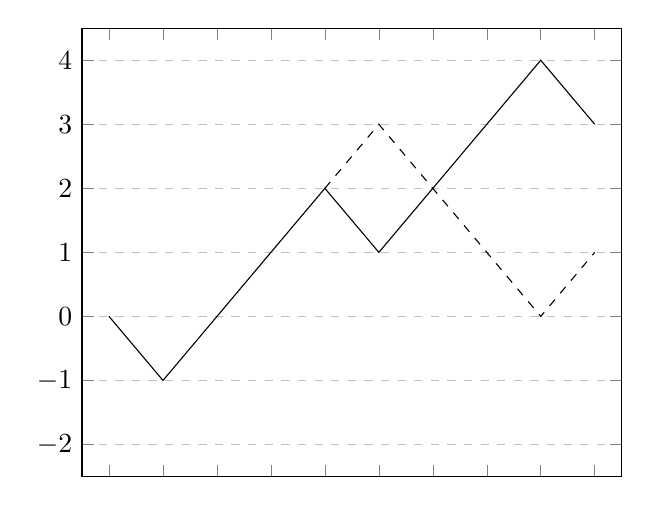
\begin{tikzpicture}
	\begin{axis}[ymajorgrids=true, grid style={line width=.3pt,  dashed}, enlargelimits={abs=0.5}, axis line style={latex-latex}, xticklabels={,},xtick={0,1,2,3,4,5,6,7,8,9}, ytick={-2,-1,0,1,2,3,4}, ymin=-2]
	\addplot[black,] coordinates { (0,0) (1,-1) (2,0) (3,1) (4,2) (5,1) (6,2) (7,3) (8,4) (9,3)}; 	
	\addplot[black, dashed] coordinates {(4,2) (5,3) (6,2) (7,1) (8,0) (9,1)};
\end{axis}
\end{tikzpicture}
\end{center}
\caption{Example of a reflected simple random walk for $a=2$}
\end{figure}

Consider the SRW on $\mathbb{Z}$: 

\begin{prop}[]
Let $k\geq 0$ even, $a\geq1$ odd: $\mathbb{P}_{0} \left[ \max_{0 \leq m \leq k} X_m \geq a \right] = \mathbb{P}_{0} \left[ |X_k|\geq a \right]  $
\end{prop}
\begin{proof}
	Define $H_a= \min\{n \geq 1: X_n =a\}$, this is a stopping time.
	\begin{align}
		\mathbb{P}_{0} \left[ \max_{0 \leq m \leq k}X_m \geq a \right] = \mathbb{P}_{0} \left[ H_a \leq k \right] = \mathbb{P}_{0} \left[ X_k > a \right]  + \mathbb{P}_{0} \left[ H_a \leq k, X_k < a \right] 
		\end{align}
		Now our goal is to show the term on the right is equal to $\mathbb{P}_{0} \left[ X_k > a \right] $, as $2\mathbb{P}_{0} \left[ X_k > a \right] = \mathbb{P}_{0} \left[ |X_k| >a \right] $ by symmetry. We can go from $>$ to $\geq$ because $a$ is even and $k$ is odd. At this point we note that $X_{H_a +n} \sim a + (a-X_{H_a +n}) = 2a - X_{H_a +n}$. Geometrically, this means that if we only look at the walk after hitting $a$, the walk has the same distribution if we inverse the direction of each step: 'looking at the path after hitting $a$, we cannot tell if it is the normal or the inverted step walk'.
	\begin{align}
		\mathbb{P}_{0} \left[ H_a \leq k, X_k < a \right] &= \sum_{m=0}^{k} \mathbb{P}_{0} \left[ X_k < a, H_a = m \right] = \sum_{m=0}^{k} \mathbb{P}_{a} \left[ X_{k-m} < a \right] \mathbb{P}_{0} \left[ H_a = m \right]  \\
		&= \sum_{m=0}^{k} \mathbb{P}_{a} \left[ X_{k-m}>a \right] \mathbb{P}_{0} \left[ H_a = m \right] = 
			 \sum_{m=0}^{k} \mathbb{P}_{0} \left[ X_{k-m}>a, H_a =m \right] \\
		&= \mathbb{P}_{0} \left[ X_k >a, H_a \leq k \right] = \mathbb{P}_{0} \left[ X_k > a \right]  
	 \end{align}
	
\end{proof}


\noindent
\textbf{Conclusion} Now we have properly defined a Markov Chain, shown its existence, and introduced some concepts to help classify different types of chains. Importantly, we have also introduced the transition probability framework. 


